\documentclass[tikz,border=10pt]{standalone}
\usepackage[utf8]{inputenc}
\usepackage[T1]{fontenc}
\usepackage{tikz}
\usetikzlibrary{shapes.geometric, arrows.meta, positioning, fit, backgrounds}

\begin{document}

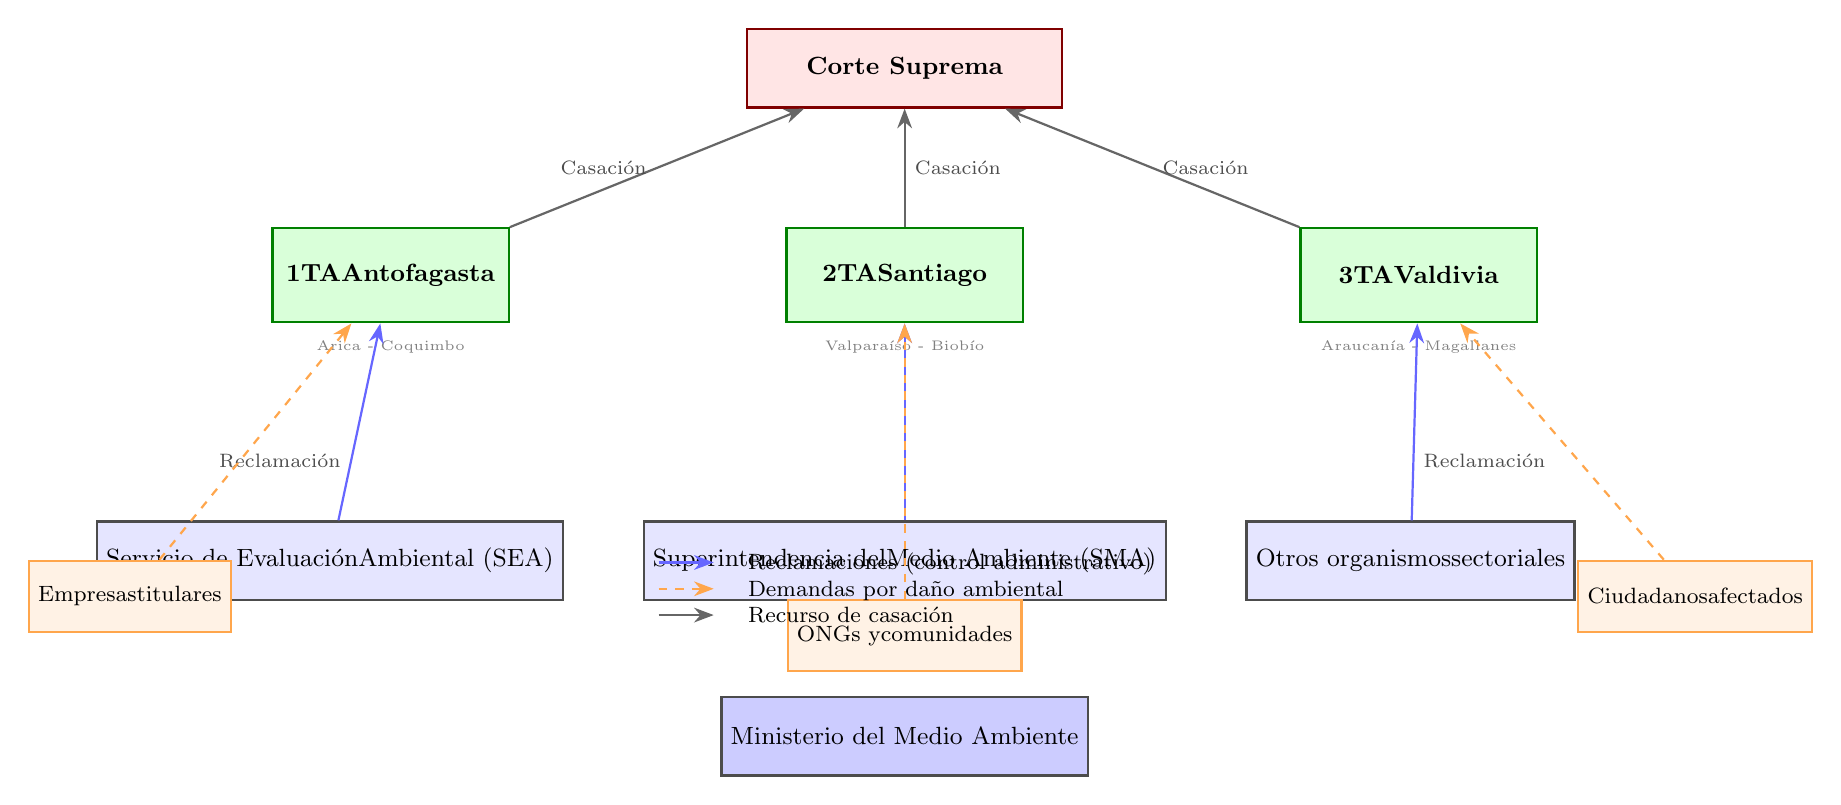
\begin{tikzpicture}[
    node distance=1.2cm and 2cm,
    box/.style={rectangle, draw=black!70, fill=blue!10, thick,
                minimum width=3.5cm, minimum height=1cm,
                text centered, font=\small},
    tribunal/.style={rectangle, draw=green!50!black, fill=green!15, thick,
                     minimum width=3cm, minimum height=1.2cm,
                     text centered, font=\small\bfseries},
    corte/.style={rectangle, draw=red!50!black, fill=red!10, thick,
                  minimum width=4cm, minimum height=1cm,
                  text centered, font=\small\bfseries},
    actor/.style={rectangle, draw=orange!70, fill=orange!10, thick,
                  minimum width=2.5cm, minimum height=0.9cm,
                  text centered, font=\footnotesize},
    arrow/.style={-{Stealth[length=2.5mm]}, thick, draw=black!60},
    label/.style={font=\scriptsize, text=black!70}
]

% Nivel superior - Corte Suprema
\node[corte] (cs) {Corte Suprema};

% Nivel de Tribunales Ambientales
\node[tribunal, below left=1.5cm and 3cm of cs] (1ta) {1TA\\Antofagasta};
\node[tribunal, below=1.5cm of cs] (2ta) {2TA\\Santiago};
\node[tribunal, below right=1.5cm and 3cm of cs] (3ta) {3TA\\Valdivia};

% Jurisdicciones
\node[below=0.1cm of 1ta, font=\tiny, text=gray] {Arica - Coquimbo};
\node[below=0.1cm of 2ta, font=\tiny, text=gray] {Valparaíso - Biobío};
\node[below=0.1cm of 3ta, font=\tiny, text=gray] {Araucanía - Magallanes};

% Nivel de organismos administrativos
\node[box, below=2.5cm of 2ta] (sma) {Superintendencia del\\Medio Ambiente (SMA)};
\node[box, left=1cm of sma] (sea) {Servicio de Evaluación\\Ambiental (SEA)};
\node[box, right=1cm of sma] (otros) {Otros organismos\\sectoriales};

% Ministerio
\node[box, below=1.2cm of sma, fill=blue!20] (mma) {Ministerio del Medio Ambiente};

% Actores
\node[actor, below left=3cm and 0.5cm of 1ta] (emp) {Empresas\\titulares};
\node[actor, below=3.5cm of 2ta] (ong) {ONGs y\\comunidades};
\node[actor, below right=3cm and 0.5cm of 3ta] (ciu) {Ciudadanos\\afectados};

% Flechas de apelación
\draw[arrow] (1ta) -- node[label, left, pos=0.5] {Casación} (cs);
\draw[arrow] (2ta) -- node[label, right, pos=0.5] {Casación} (cs);
\draw[arrow] (3ta) -- node[label, right, pos=0.5] {Casación} (cs);

% Flechas de reclamación
\draw[arrow, blue!60] (sea) -- node[label, left, pos=0.3] {Reclamación} (1ta);
\draw[arrow, blue!60] (sma) -- (2ta);
\draw[arrow, blue!60] (otros) -- node[label, right, pos=0.3] {Reclamación} (3ta);

% Flechas de demanda por daño
\draw[arrow, orange!70, dashed] (emp) -- (1ta);
\draw[arrow, orange!70, dashed] (ong) -- (2ta);
\draw[arrow, orange!70, dashed] (ciu) -- (3ta);

% Leyenda
\node[below=5.5cm of cs, font=\footnotesize] (ley) {
    \begin{tabular}{ll}
    \tikz\draw[arrow, blue!60] (0,0) -- (0.7,0); & Reclamaciones (control administrativo) \\
    \tikz\draw[arrow, orange!70, dashed] (0,0) -- (0.7,0); & Demandas por daño ambiental \\
    \tikz\draw[arrow] (0,0) -- (0.7,0); & Recurso de casación \\
    \end{tabular}
};

\end{tikzpicture}

\end{document}
